\documentclass[10pt]{article}
\usepackage[margin=0.72in]{geometry}
\usepackage[T1]{fontenc}
\usepackage{lmodern}
\usepackage{microtype}
\usepackage{booktabs}
\usepackage{tabularx}
\usepackage{graphicx}
\usepackage{xcolor}
\usepackage{enumitem}
\usepackage{hyperref}
\hypersetup{colorlinks=true,linkcolor=black,urlcolor=blue!55!black}
\setlist{nosep,leftmargin=*}
\setlength{\parindent}{0pt}
\setlength{\parskip}{4pt}
\definecolor{accent}{HTML}{173F5F}
\newcommand{\result}[1]{\textbf{\color{accent}#1}}

\title{\vspace{-1.2cm}\textbf{BTC--Nasdaq Cross-Market Signal Validation}\\
\large Leakage-aware event research with realistic MNQ execution}
\author{Validation rebuild: Robert Mazurczak\\
Original research: Robert Mazurczak and Alexandra Samuseva (\href{https://github.com/AlexSamuseva}{@AlexSamuseva})}
\date{16 September 2026}

\begin{document}
\maketitle

\begin{abstract}
This study asks a narrow question: \emph{do BTC-derived features improve prediction of Nasdaq futures event returns over a comparable NQ-only momentum baseline after costs?} We rebuild an earlier notebook backtest as a causal event pipeline. Features are known at the close of minute $t$, execution occurs at the open of $t+1$, positions do not overlap, contract rolls and discontinuities are excluded, and all model choices are made from purged expanding walk-forward predictions. The period 1 January--12 May 2026 is opened only after the configuration and source hashes are locked. The final test contains 824 candidate events. The BTC--NQ rule and Random Forest have positive point estimates, but their 95\% block-bootstrap confidence intervals include zero. The NQ-only baseline and NQ-only Logistic Regression are net negative. \result{The prespecified positive-edge criterion is not met.} The useful result is a reproducible model-validation case study, not a claim of a deployable trading strategy.
\end{abstract}

\section*{Research question and decision rule}
The candidate universe consists of large 15-minute NQ momentum impulses during the US cash session. Four levels are compared: an NQ momentum baseline, a BTC--NQ agreement rule, Logistic Regression, and a constrained Random Forest. A separate NQ-only Logistic Regression is retained as an ablation: it directly measures whether BTC variables add predictive value.

A positive edge may be declared only when the locked final test has at least 50 trades, positive net P\&L, and a positive lower bound for a 95\% day-block bootstrap confidence interval of mean net P\&L. Profit factor is capped for reporting and cannot override the minimum sample rule. Under this decision rule, no evaluated strategy supports a positive-edge claim.

\begin{table}[h]
\centering
\small
\begin{tabular}{lrrrrl}
\toprule
Final strategy & Trades & Gross USD & Net USD & Mean USD & 95\% CI, mean USD \\
\midrule
NQ momentum baseline & 824 & 2,149.50 & -322.50 & -0.39 & [-8.62, 8.49] \\
BTC--NQ rule & 413 & 4,136.50 & 2,897.50 & 7.02 & [-5.35, 19.49] \\
LogReg, NQ only & 803 & 1,782.50 & -626.50 & -0.78 & [-9.21, 8.05] \\
LogReg, cross-market & 742 & 2,610.50 & 384.50 & 0.52 & [-8.54, 10.13] \\
Random Forest, cross-market & 55 & 1,795.00 & 1,630.00 & 29.64 & [-20.83, 79.09] \\
\bottomrule
\end{tabular}
\caption{Locked final-test results for one MNQ contract after the configured round-trip cost.}
\end{table}

\newpage
\section{Audit of the legacy backtest}
The original notebooks were useful exploratory work, but their headline metrics cannot be interpreted as executable performance. They are preserved under \texttt{legacy/} for attribution and auditability; they are explicitly not a source of truth.

\subsection*{Material failure modes}
\begin{itemize}
  \item \textbf{Costs dominated the apparent edge.} One notebook reported 14,554 NQ points from 258,207 trades, only 0.056 point per trade. The later ML notebook reported 1,599 points from 21,188 trades, 0.075 point per trade. Both averages are below a single MNQ tick of 0.25 point before commission.
  \item \textbf{Overlapping candidate returns were summed.} A sequence of neighboring signal bars could contribute several labels that represented the same market move, inflating sample size and invalidating P\&L aggregation.
  \item \textbf{Execution used information unavailable at the fill.} Filling at a close that was required to compute the signal creates look-ahead execution. The rebuilt engine enters at the next bar's open.
  \item \textbf{Time handling was not exchange-safe.} A fixed UTC offset cannot represent US daylight-saving transitions. The rebuild localizes NQ source timestamps to \texttt{America/Chicago}, converts through UTC, and evaluates the session in \texttt{America/New\_York} using CME Equity trading dates.
  \item \textbf{Contract changes and missing bars were not guarded.} Events that cross a roll, timestamp gap, day boundary, or session end are now rejected.
  \item \textbf{Selection and evaluation were mixed.} Thresholds and models were compared on the final period, and some rolling experiments learned from labels inside that period. The rebuild permits selection only from out-of-fold pre-2026 predictions.
  \item \textbf{Sharpe annualization was inconsistent.} Per-trade observations and a hard-coded two-year factor were mixed. The maintained report uses daily net P\&L and $\sqrt{252}$, while also showing bootstrap uncertainty.
\end{itemize}

An intermediate replay also revealed a ranking defect: configurations with \texttt{profit\_factor = inf} could receive an infinite robustness score despite only one to three validation trades. This rebuild makes 50 validation trades a hard feasibility constraint; the capped profit factor is descriptive only.

\section{Data and economic assumptions}
BTCUSDT USD-M one-minute bars are public Binance data. NQ one-minute bars are a local IBKR-derived, stitched contract series and are not redistributed. The repository contains a schema, a Binance downloader, and synthetic fixtures instead of proprietary data.

MNQ economics use the official contract multiplier of \$2 times the index, a 0.25-point minimum tick, and a \$0.50 tick value. See the \href{https://www.cmegroup.com/markets/equities/nasdaq/micro-e-mini-nasdaq-100.html}{CME product page}. The locked conservative scenario assumes one tick of slippage per side and \$1 commission per side, giving a \$3.00 round trip. Broker commissions remain configurable and should be checked against the current \href{https://www.interactivebrokers.com/en/pricing/commissions-futures.php}{IBKR futures schedule}.

\newpage
\section{Causal event protocol}
At minute $t$, all features are calculated from bars whose closes are available no later than $t$. An event is the first bar on which the absolute 15-minute NQ return crosses a training-fitted 70th-percentile threshold (8.1193 bps). The direction is the sign of that return. Entry is the open of $t+1$; exit is the open 30 minutes after entry. A global cooldown enforces one open position at a time.

An event is discarded if any required feature is missing, any one-minute timestamp is absent, the NQ contract identifier changes, entry and exit do not share a session date, or the exit is later than 16:00 New York time. This turns the research unit from a highly overlapping bar into a trade-like event with a uniquely attributable outcome.

\subsection*{Feature sets}
The NQ-only set contains 5/15/30-minute momentum, 15/60-minute volatility, 14-minute ATR, RSI, and cyclical time-of-day features. The cross-market set adds BTC momentum and volatility, exact rolling 55-minute Spearman correlation, a 55-minute directional hit ratio, and the BTC-minus-NQ momentum spread. All rolling state resets after data or contract discontinuities.

\subsection*{Labels and costs}
For the event direction $d \in \{-1,1\}$, gross points are
\[
  \mathrm{points}_i = d_i(P^{\mathrm{exit}}_i-P^{\mathrm{entry}}_i).
\]
Gross USD equals points times \$2. Net USD subtracts the full round-trip cost. The binary label is one only when net USD is positive. This makes the classifier answer a tradable question---whether the already-defined directional event clears costs---rather than predicting an arbitrary next-bar sign.

\section{Walk-forward validation and model controls}
Expanding quarterly folds begin in 2024Q4. Each training sample must precede the validation boundary by the configured 60-minute purge, which exceeds the maximum 30-minute holding horizon. Standardization is fitted inside each Logistic Regression fold. Random Forest permutation importance and Logistic Regression coefficients are aggregated from fold-local estimators; no final-test observation participates.

The Logistic Regression regularization and constrained Random Forest depth/leaf size are fixed in configuration. Probability thresholds in \{0.45, 0.50, 0.55, 0.60, 0.65, 0.70\} are ranked using OOF events only and must retain at least 50 trades. The trial ledger records all feasible comparisons; the manifest reports 20 research trials. Selection-bias context follows Bailey and L\'opez de Prado's \href{https://papers.ssrn.com/sol3/papers.cfm?abstract_id=2460551}{Deflated Sharpe Ratio} and \href{https://papers.ssrn.com/sol3/Papers.cfm?abstract_id=2326253}{Probability of Backtest Overfitting}. The reported DSR is an explicitly approximate diagnostic, not a p-value.

\newpage
\section{Validation evidence}
The OOF NQ baseline lost \$6,369.50 over 2,500 events; the BTC--NQ rule lost \$4,183 over 1,187 events. Both Logistic Regression selections were negative after costs. The Random Forest chose a 0.55 threshold and earned \$1,102 over 356 validation trades, but its mean-net 95\% CI was [-\$7.88, \$14.00]. Thus, even the selected model did not establish a stable validation edge.

\begin{figure}[h]
\centering
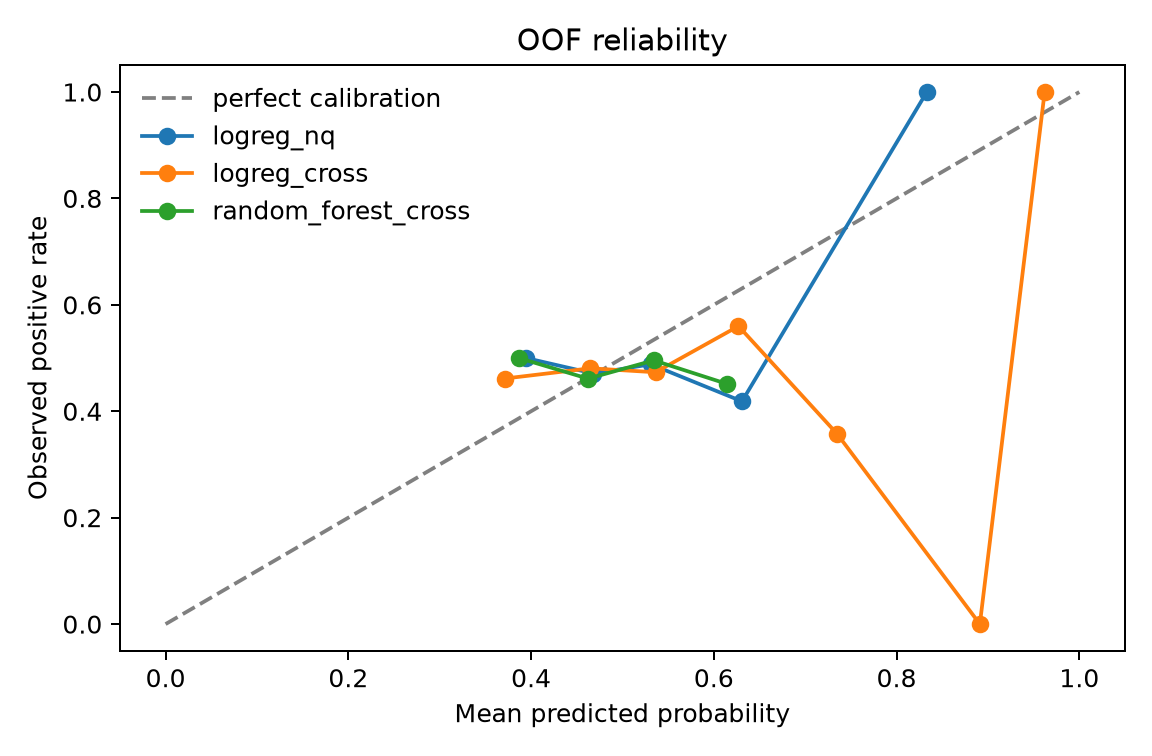
\includegraphics[width=0.84\textwidth]{../outputs/portfolio/reliability_oof.png}
\caption{Out-of-fold reliability. Brier scores were 0.2515 (NQ LogReg), 0.2535 (cross-market LogReg), and 0.2499 (cross-market RF), close to an uninformative balanced forecast.}
\end{figure}

The cross-market Logistic Regression did not improve calibration over the NQ-only ablation. Coefficient and permutation-importance magnitudes are included in the machine-readable manifest rather than interpreted causally: correlated rolling variables, non-stationarity, and low signal-to-noise make such interpretations fragile.

\subsection*{Locked research state}
The versioned manifest stores sanitized configuration, data range, event threshold, feature lists, OOF threshold selections, trial count, a SHA-256 hash of the maintained package, and a hash of the locked setting. The final command refuses a changed configuration or source tree and refuses a second final evaluation unless an explicit override is supplied. The published final result hash is retained in the manifest.

\newpage
\section{Final test}
The final interval produced 824 eligible events. Figure~\ref{fig:final} shows mean net USD per accepted trade. Positive bars are point estimates, not evidence of a positive population mean.

\begin{figure}[h]
\centering
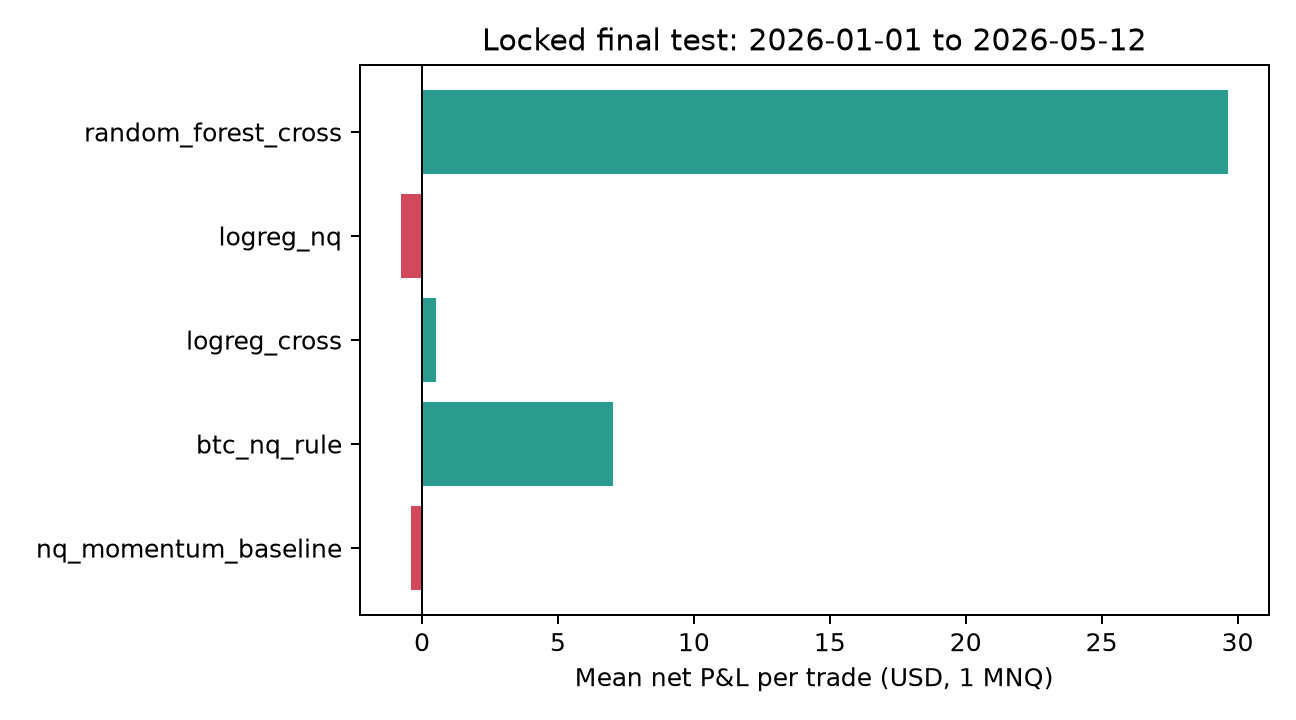
\includegraphics[width=0.88\textwidth]{../outputs/portfolio/final_test_snapshot.png}
\caption{Locked final-test mean net P\&L per trade. All strategy confidence intervals include zero.}
\label{fig:final}
\end{figure}

\section{Interpretation, drift, and limitations}
The BTC--NQ rule and cross-market Random Forest are directionally interesting, but neither passes the uncertainty gate. The Random Forest result is particularly fragile: 55 trades barely clear the minimum and its confidence interval is very wide. The cross-market Logistic Regression adds no practical value over its NQ-only ablation. The correct conclusion is \result{no validated positive edge}; the positive estimates remain inconclusive follow-up hypotheses.

Population Stability Index diagnostics do not show an obvious catastrophic covariate shift. The largest final-versus-pretest PSI was 0.11 for rolling BTC--NQ Spearman correlation, followed by 0.06 for directional hit ratio and 0.05 for NQ 60-minute volatility. These diagnostics are descriptive: a low PSI cannot establish label stability or model correctness.

\subsection*{Limitations}
\begin{itemize}
  \item The study uses one stitched NQ data source and cannot independently verify vendor corrections, roll construction, or bid/ask history.
  \item Slippage is a configurable fixed scenario, not a market-impact model; latency, queue position, spread variation, partial fills, and exchange fees are simplified.
  \item The event family and feature family reflect prior exploration. Trial counting and approximate DSR make that risk visible but cannot fully reconstruct every human research decision.
  \item The final interval covers roughly four months. Day-block bootstrap preserves same-day dependence but cannot create unobserved regimes.
  \item Classification calibration near 0.5 is weak. Feature importance is predictive and fold-specific, not structural or causal evidence linking BTC to NQ.
\end{itemize}

\section{Reproducibility and conclusion}
The maintained interface is:
\begin{verbatim}
python -m cross_market.run --config configs/research.yaml --stage validation
python -m cross_market.run --config configs/research.yaml --stage final
\end{verbatim}
The first command creates OOF diagnostics and the lock; the second verifies the lock before opening the final period. CI runs lint, formatting, type checks, unit/integration tests, a notebook smoke test, and committed-artifact checks. Public data may be downloaded; the local NQ file must conform to the documented schema.

The project demonstrates a defensible research outcome even without alpha: causal timing, event construction, realistic contract costs, purged walk-forward model selection, probabilistic calibration, drift analysis, selection-bias awareness, and an immutable final-test audit trail. The hypothesis that BTC features create a robust after-cost NQ edge is not established by this sample. Any follow-up must begin as a new, versioned hypothesis with a new untouched evaluation period.

\vfill
\footnotesize\textbf{Artifact identity.} Locked setting hash: \texttt{ac32ede2a2acde76b7d856e8874dfe4f01da42f2738cfd6271e5321e359e75e6}. Final result SHA-256: \texttt{c9ce293cde804d811de0675508e7bf045b39ecae567a8e8116119b0c6df2a198}.

\end{document}
